\documentclass[12pt]{article}
\usepackage{tikz}
\usetikzlibrary{shapes,snakes}
\usetikzlibrary{arrows,automata}
\usepackage{algorithm}
\usepackage{algorithmic}
\usepackage{graphicx} 
\usepackage{fancybox}
\usepackage{setspace}  
\usepackage[colorlinks,linkcolor=blue,citecolor=magenta]{hyperref}
\usepackage{enumerate} 
\usepackage{amsthm,amssymb,amsmath}
\usepackage{indentfirst}
\usepackage{listings}
\usepackage{alltt}
\usepackage{clrscode}
\usepackage{mathtools}
\usepackage{float}
\renewcommand{\algorithmiccomment}[1]{// #1}
\floatstyle{plain}

\newtheorem{theorem}{Theorem}[section]
\newtheorem{corollary}{Corollary}[section]
\newfloat{program}{h}{lop}[section]
\floatname{program}{}
\begin{document}

\title{Initial Value Computation}
\author{}
\date{\today}
\maketitle
\newcommand{\dom}{\textsf{DBT-dom}}
\newcommand{\multip}{\textsf{DBT-multip}}
\newcommand{\InputVars}{\textsf{InputVars}}
\newcommand{\OutputVars}{\textsf{OutputVars}}
\newcommand{\Rel}{\textsf{Rel}}
\newcommand{\Ext}{\textsf{Ext}}

\section{Defining DBT-domains}
\label{sec:definingdomains}
In this draft we want to explain the notion of DBT-domains in DBToaster calculus \cite{1}. DBToaster uses query language AGCA(which is stands for AGgregation CAlculus). 
AGCA expressions are built from constants, variables, relational atoms, aggregate sums (Sum), conditions, and variable assignments ($\gets$) using ``+''  and ``$\cdot$''. The abstract syntax can be given by the EBNF:
\begin{equation}
\label{def:agca}
q\coloneqq  q\cdot q | q + q|v \gets q |v_{1}\theta v_{2}|R(\vec{y})|\text{c}|\text{v}|(M[\vec{x}][\vec{y}]\coloneqq q)
\end{equation}
The above definition can express all SQL statements. Here $v$ denotes variables, $\vec{x},\vec{y}$ tuples of variables, $R$ relation names, $c$ constants, and $\theta$ denotes comparison operations $(=,\neq, >, \geq, <, \text{ and }\leq)$.
 ``+'' represents unions and ``$\cdot$'' represents joins. Assignment operator($\gets$) takes an query and assigns its result to a variable($v$). A map $M[\vec{x}][\vec{y}]$ is a subquery with some input($\vec{x}$) and output($\vec{y}$) variables. It can be seen as a nested query that for the arguments $\vec{x}$ produces the output $\vec{y}$, it is not defined in \cite{1} but we added here for the purpose of this work.

The DBT-domain of a variable is the set of values that it can take. The DBT-domain of all the variables in a query expression can easily be computed recursively if some rules are respected. We will use through out the entire paper the notation of $\text{\dom{}}_{\vec x}(q)$ for the DBT-domain of a set of variables, where $q$ is the given query and $\vec x$ is a vector representing the variables(not necessarily present in the expression $q$). We will start by saying the $\vec x=\langle x_1,x_2,x_3,\cdots,x_n\rangle$ will be the schema of all the variables 
and that $\vec c=\langle c_1,c_2,c_3,\cdots,c_n\rangle$ will be the vector of all constants, that will match the schema presented by $\vec x$. It is not necessary that $\vec{x}$  has the same schema as the given expression. We will give the definition of $\dom{}_{\vec x}(R(\vec y))$:

\begin{equation}
\label{def:relation}
\dom{}_{\vec x}(R(\vec y))=\bigg\{\vec c\,\Big|\,\sigma_{\forall x_i\in(\vec{y}): x_{i}=c_{i}}R(\vec y)\not= \const{NULL}\bigg\}
\end{equation}

Thus, we can evaluate $\text{\dom}_{\vec{x}}$ for a broader range of $\vec{x}$ and it is not restricted by the schema of the input query expression. In such cases the \dom{} is infinite as the not presenting variables in the query can take any value.

\begin{equation}
\text{\dom{}}_{\vec{x}}(v_{1}\theta v_{2})=\bigg\{\vec{c}\,\Big|\,\forall i,j:(v_{1}=x_{i}\land v_{2}=x_{j})\Rightarrow c_{i}\theta c_{j}\bigg\}
\end{equation}

The DBT-domain of a comparison is infinite.

For the join operator we can write:
\begin{equation}
\label{def:join}
\text{\dom{}}_{\vec{x}}(q_{1}\cdot q_{2})=\{\vec{c}\,|\vec{c}\in\text{\dom{}}_{\vec{x}}(q_{1})\land\vec{c}\in\text{\dom{}}_{\vec{x}}(q_{2})\}
\end{equation}
while for the union operator the DBT-domain definition is very similar:
\begin{equation}
\label{def:plus}
\text{\dom{}}_{\vec{x}}(q_{1}+ q_{2})=\{\vec{c}\,|\vec{c}\in\text{\dom{}}_{\vec{x}}(q_{1})\lor\vec{c}\in\text{\dom{}}_{\vec{x}}(q_{2})\}
\end{equation}
\begin{eqnarray}
\dom{}_{\vec x}(constant)=\Big\{\vec c\Big\}\label{def:const}\\
\dom{}_{\vec x}(variable)=\Big\{\vec c\Big\}\label{def:var}
\end{eqnarray}
In \eqref{def:const} and \eqref{def:var}  $\vec{c}$ stands for all possible tuples match schema of $\vec{x}$, so the DBT-domains in these two cases are infinite. 
Finally, we can give a formalism for expressing the DBT-domain of a variable that will participate in an assignment operation:

\begin{equation}
\label{assign2}
\text{\dom{}}_{\vec{x}}(v\gets q_{1})=\Big\{\vec{c}\Big|\vec{c}\in\text{\dom{}}_{\vec{x}}(q_{1})\land \big(\forall i: (x_{i}=v)\Rightarrow(c_{i}=q_{1})\big)\Big\}
\end{equation}
In fact using implication operator in the above definition allows us to extend the $\vec{x}$ to whatever vector we want, as we already said the schema of $\vec{x}$ is not necessarily the same as the schema of $q$. %Here is a mathematical reformulation of \eqref{assign1}:
We can define the DBT-domain of a map(for map's definition refer to \cite{1}, \cite{2}) as follow:
\begin{equation}
\label{def:map}
\text{\dom}_{\vec{w}}(map[\vec{x}][\vec{y}])=\{\vec{c}|\vec{c}\in\text{\dom}_{\vec{w}}(\vec{x}\cup\vec{y})\}
\end{equation}
We define function \Ext{}  to extend(shrink) the schema of a DBT-domain, $a$ as input with schema $\vec{y}$:
\begin{equation}
\label{def:ext}
\text{\Ext}_{\vec{x}}(a_{\vec{y}})=\{\vec{c}|\sigma_{\forall i\,y_{i}\in\vec{x}:(y_{i}=c_{i})}a\neq \text{NULL}\}
\end{equation}
In \eqref{def:ext} we can consider $a$ as relation since it is a set and using the relational algebra on it. 
It is clear that if $\vec{x}\cap\vec{y}\neq\vec{x}$ it produces an infinite DBT-domain. 

\section{DBT-domain computation}\label{DBT-domain}

We are trying to compute the DBT-domain of variables that appear in queries. This computation is performed on the parse tree. We can traverse the tree in post order, first visiting the leaves that are represented by some relations and afterwards visiting the parent nodes and combining the relations of the children nodes. Using this technique we are trying to compute the DBT-domains, but also the vector $\vec x$ of all the variables defined in that query.

The intuition behind the algorithm is simple. For computing the DBT-domain of a node we first compute the DBT-domain of its left child and according to the operator of the node itself we decide how to send the information from left child to right child, and then the DBT-domain of the right child.

The algorithm needs as inputs the root of the tree and a structure that must be previously defined and returns a structure that contains the vector of variables($\vec{x}$) and the DBT-domains for each variable defined in the vector(\dom). This structur is called $NodeAttribute$ and it looks like:

\begin{program}
\begin{alltt}
struct \{
x: the vector of all the variables 
dom: the DBT-domains of all the variables
\}
\end{alltt}
\caption{$NodeAttribute$}
\label{struct}
\end{program}
In Algorithm \ref{alg1} we define function \textsf{computeDBT-Domains} which helps us to compute the DBT-domains for variables within a given query. When invoking the function, we pass as arguments of the function, the root of the parse tree and a structure which will have the vector of variables and the DBT-domain of the variables as nil, \textsf{computeDBT-Domain}$(root,s)$.
\par
In Algorithm~\ref{alg1} we have a variable $node$ which represents a node in the parse tree. It has 2 children which can be accessed by fields $left, right$. Also each node has a type field, which can be accessed by $type$. A type of a node can be any of different types in definition~\eqref{def:agca}. For handling map types we suppose that each node that represents a map has a child (accessible via filed $child$, line~\ref{lst:child}) which points to the map itself (i.e. Figure~\ref{fig:map}). In other words each map introduces an intermediate node in the tree structure, this node has two fields $\vec{x},\vec{y}$ to represent input and output DBT-domain of the map. 

\begin{algorithm}[H]
\caption{computeDBT-Domains($node$,$s$)} 
\label{alg1}
\textbf{Input:} $node$ as the root of the tree to be traversed, and $s$ is of type $NodeAttribute$ \\
\textbf{Output:}  $result$ of type $NodeAttribute$ that contains vector of variables $\vec x$ and the DBT-domains of each variable $\dom{}_{\vec x}(query)$
\begin{algorithmic}[1]
\IF{$node.type=$``+''}
\STATE  $s_{1}\gets$ computeDBT-Domain($node.left, s$)
\STATE  $s_{2}\gets$ computeDBT-Domain($node.right, s$)
\STATE  $result.\vec{x}\gets s_{1}.\vec{x} \cup s_{2}.\vec{x}$ %\COMMENT{this will compute the vector for all the variables, both from the right and left node}
\STATE  $result.dom\gets \text{\dom}_{result.\vec x}(s_{1}.dom)\cup\text{\dom}_{result.\vec x}(s_{2}.dom)$
\ELSIF{$node.type=$``*''}
\label{line:join1}
\STATE  $s_{1} \gets \text{computeDBT-Domain}(node.left, s)$\label{line:join2}
\STATE $result\gets$ computeDBT-Domain$(node.right, s_{1})$
\ELSIF{$node.type=$``Map''}
\label{lst:map}
\STATE $node.\vec{x}\gets\text{\dom}_{s.\vec{x}}(s.dom)$
\STATE $node.\vec{y}\gets$computeDBT-Domain$(node.child,s)$\label{lst:child}
\STATE $result.\vec{x}\gets s.\vec{x}$
\STATE $result.dom\gets node.\vec{y}$
\ELSE 
\label{line10}
\STATE $result.\vec{x}\gets s.\vec{x} \cup \{\text{Var$(node)$}\}$\label{lst:setofallvar}
\STATE $result.dom\gets \text{\Ext}_{result.\vec{x}}(s.dom)\cap\text{\dom}_{result.\vec{x}}(node)$\label{line2}
\ENDIF
\RETURN $result$
\end{algorithmic}
\end{algorithm}
The order of Algorithm \ref{alg1} is $O(n\cdot P)$ where $n$ is the number of nodes in the parse tree and $P$ is the time needed for any rule of \dom{}'s computation, according to previous section. Clearly this algorithm visits each node only one time. \par

Algorithm \ref{alg1} all types of nodes: union nodes, join nodes, map nodes and all other type of nodes. In addition to nodes, we have three types of leaves: simple relations $R(\vec y)$, inequalities $v_{1}\theta v_{2}$ and assignment relations $v \gets q$. A union node or a join node will always have two children, therefore the line \ref{line10} will be executed when a leaf is visited. When a map node is encountered, line~\ref{lst:map}, then the algorithm should produce the DBT-domain of input and output variables. In line \ref{line2} we use function \Ext{} to extend the schema of the input DBT-domain to a broader schema of $result.\vec{x}$. We use this for extending a DBT-domain regarding to a new schema vector $result.\vec x$. 

In line~\ref{lst:setofallvar} we want to compute the set of variables in the node. Since the node is a leaf, it can represents a relation, an assignment or a comparison. We can compute the set of variables in a leaf with the following rules:
\begin{align}
\text{Var}(R(\vec{y}))&=\{y_{1},\cdots,y_{n}\}\\
\text{Var}(v_{1}\theta v_{2})&=\{v_{1},v_{2}\}\\
\text{Var}(v\gets q_{1})&=\{v\}\cup\text{Var}(q_{1})
\end{align}
\begin{figure}[htbp]
\begin{center}
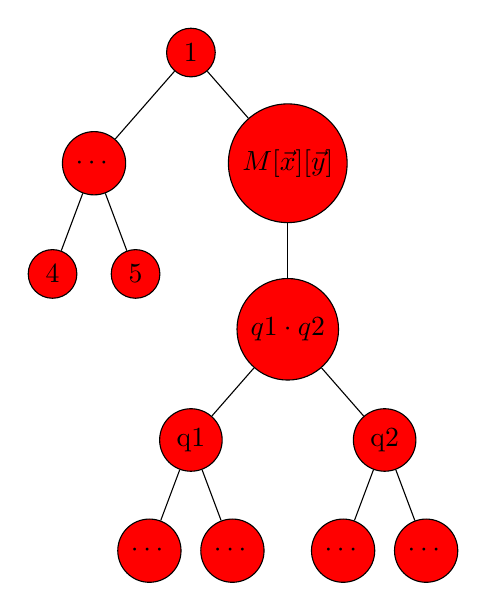
\begin{tikzpicture}%[level/.style={sibling distance=40mm,level distance=15mm}]
[level 1/.style={circle, draw,scale=1.0, fill=red,
    level distance=40pt, sibling distance=70pt},
    level 2/.style={circle, draw, scale=1.0,
    level distance=60pt, sibling distance=70pt},
    level 3/.style={circle, draw, scale=1.0,
    level distance=40pt, sibling distance=70pt},
    level 4/.style={circle, draw, scale=1.0,
    level distance=40pt, sibling distance=30pt}]
    \tikzstyle{every node}=[circle,draw,fill=red]
    \node[] (a){1}
        child { 
            node [](b){$\cdots$}
            child[sibling distance=30pt,level distance=40pt]{
            	node{4}
            }
            child[sibling distance=30pt,level distance=40pt]{
            	node{5}
            }
        }
        child{ 
        		node[](c){$M[\vec{x}][\vec{y}]$}
        		child{
        			node[](d){$q1\cdot q2$}
        			child{
        				node[](f){q1}
        				child{node[](g){$\cdots$}}
        				child{node(h){$\cdots$}}
        				}
        			child{
        				node[](i){q2}
        				child{node[](j){$\cdots$}}
        				child{node(k){$\cdots$}}
        				}
        			}
		};
\end{tikzpicture}
\end{center}
\caption{Tree representation}
\label{fig:map}
\end{figure}

The algorithm starts with node 1, which represents the root of the parse tree. It recursively goes through each of the leaves, therefore constructs the variable vector and also the DBT-domain for each variable.
	
We have mentioned that besides map nodes, there are two more types of intermediate nodes: the union node and the join node. When a union node is met, then it is known that DBT-domains of variables will not pass over this operator and for that the variables and their DBT-domains, which were obtained in the parent, will be passed to each of this node's children. Thus it applies the distribution rule of the join operator over the union operator. For example if we have $ q_{1} * (q_{2} * q_{3} + q_{4} * q_{5}) \equiv q_{1} * q_{2} * q_{3} + q_{1} * q_{4} * q_{5}$, the variables and DBT-domain obtained for $q1$ will be passed both to $q_{2}*q_{3}$ and $q_{3}*q_{4}$, without modifying any of the DBT-domains, regarding that some DBT-domains may change on one branch, for example $q2*q3$. For the other type of node, the join node, the passing of DBT-domains is allowed, and therefore a DBT-domain can be refined by the relation on the right side of the parent node.
	
Every time the algorithm encounters a map then it will create the DBT-domain for that specific map. Here we can make a difference between input and output variables, because the DBT-domain of input variables is dependent on the DBT-domains of output variables from the left side of the map's parent node, and the DBT-domain of the output variables are going to be produced by the children of the map's node. %All this information will be stored in a global variable which can be easily accessed.

A node which is represented by a map will have only one child, because as we mentioned in the definition of the AGCA expression, a map can be defined over an expression or expressions: $M[\vec{x}][\vec{y}]\coloneqq q$
\begin{theorem}
Algorithm \ref{alg1} computes the DBT-domain of each variables and maps.
\end{theorem}

\begin{proof}
The proof is by induction on the height of the tree. The theorem is held for a tree consisting of only one node. Since this node is a simple relation and the Algorithm \ref{alg1} goes  through lines \ref{line10}-\ref{line2}. As we defined, the DBT-domain of any empty set is infinite(all possible values) so the DBT-domain is correctly computed in line \ref{line2}.

Now suppose that the Algorithm \ref{alg1} works for all the trees of a height less than $k$. We want to prove that it will work as well for trees of height $k$. Let $T$ be a tree with height $k$. If root represents a map, it has a child and we correctly computed its output DBT-domain, so the same is held for the map itself and the theorem follows in this case. Otherwise
the root should have two children. The height of both of these children should be less than $k$. So we have correctly compute the DBT-domain of the left child and its input variable. Now we have two cases, if the root node is a union node or a join node. If this is a union node then we can compute the DBT-domain of the right child independently, since no information is passed over the ``+'' in DBToaster\cite{1}. We compute the DBT-domain of the root according to definition \eqref{def:plus}. But if the root node is a join node, we have to pass the information from left child to the right child, since the right child may have some input variables which are defined in the left child. This is done in lines \ref{line:join1},\ref{line:join2}.\par
Thus in either of two cases we compute the DBT-domain of the root correctly and the theorem follows.
\end{proof}
With the above theorem we have the following corollary which helps us in section~\ref{sec:MaintainingDomainswithmultiplicity} for giving some efficient algorithm for maintaining the \dom{}s. 
\begin{corollary}
\label{col:arity0}
The multiplicity order of a tuple in the DBT-domain of a simple relation will always be greater than 0.
\end{corollary}
\section{Defining the multiplicity order of a tuple}

\subsection{Definitions}\label{Multip-def}

Having the definitions for the DBT-domains, we will try to give some insight regarding to the notion of multiplicity order of a tuple. We will start with an example relation: $$q=R(a,b)\cdot S(b,c)$$ the schema for q will have three variables $(a,b,c)$. The multiplicity of a tuple is the number of its occurrences in the relation, in other words the order of multiplicity of that tuple. The multiplicity of a tuple will increase or decrease if insertions or respectively deletions will be made to a relation. For example:
\begin{table}[ht]
\centering
\begin{tabular}{c c c c}
	R & a & b & multip order\\ [0.2ex]
	\hline
	  & $\langle $1 & 2$\rangle$ & 1 \\
	  & $\langle $1 & 3$\rangle$ & 2 \\
	  & $\langle $3 & 4$\rangle$ & 1 \\
\end{tabular}
\caption{Relation $R$}
\end{table}
\begin{table}[ht]
\centering
\begin{tabular}{c c c c}
	S & b & c & multip order\\ [0.2ex]
	%heading
	\hline
	  & $\langle $1 & 1$\rangle$ & 1 \\
	  & $\langle $2 & 2$\rangle$ & 2 \\
	  & $\langle $3 & 5$\rangle$ & 2 \\
\end{tabular}
\caption{Relation $S$}
\end{table}
\begin{table}[ht]
\centering
\begin{tabular}{c c c c c}
	$R\cdot S$ & a & b & c & multip order\\ [0.2ex]
	%heading
	\hline
	  & $\langle $1 & 2 & 2$\rangle$ & 2 \\
	  & $\langle $1 & 3 & 5$\rangle$ & 4 \\
	  & $\langle $3 & 4 & $*\rangle$ & 0 \\
	  & $\langle *$ & 1 & 1$\rangle$ & 0 \\
\end{tabular}
\caption{Relation $R\cdot S$}
\end{table}

We need to maintain the maps for certain values as long as the multiplicity order of a tuple is greater then 0. If the multiplicity order of the tuple drops to 0 then the tuple will not be taken into consideration and therefore it can be eliminated from the DBT-domains of the maps.

We need to store the multiplicity order inside each map and also way to compute the this multiplicity order of an AGCA expression. Since we substitute the subexpressions with maps, we can easily consider the relations as the maps without input variables. Also a map with input variables can be seen as a relation with a group-by clause. Input variable of a map bind some variables. Thus if we compute the map values by all different combinations of these variables, we will look up into these values and return the appropriate value according to the input variables.  

We define the function \emph{arit} which will be used to compute the multiplicity order of a tuple in a certain relation. The function will be defined on the relation and the tuple for which the multiplicity order is desired to be computed. $$arit(\text{Relation } q,\text{Tuple } t)=\text{multiplicity order of }t\text{ in the } q =\pi_{t}(q)$$ where $\pi_{t}(q)$ means the projection of relation $q$ for the tuple $t$. This function can be used for the computation of the multiplicity order of the expressions from the AGCA: $q\coloneqq q\cdot q\text{ }|\text{ }q+q\text{ }|\text{ }q \theta t\text{ }|\text{ }t\gets q\text{ }|\text{ constant}\text{ }|\text{ variable}$. However constants and variables can be eliminated from the computation because relations are of interest.

\begin{align}
arit(q_{1}\cdot q_{2},t)&=\sum\limits_{\{t_{1}\}\Join \{t_{2}\}={t}}^{}arit(q_{1},t_{1})*arit(q_{2},t_{2})\\
arit(q_{1} + q_{2},t)&=arit(q_{1},t)+arit(q_{2},t)\text{, where Schema}(q_{1})\\=\text{Schema}(q_{2})\\
arit(v_1\text{ } \theta \text{ } v_2,t)&=\begin{cases}1,& \mbox{if } v_1\theta v_2 \mbox{ is true and }v_{1}\in t \land v_{2}\in t\\
0,& \text{otherwise} \mbox{ is false} 
\end{cases}\\
arit(v\gets q,t)&=\begin{cases}0, \mbox{ if $t\setminus\{v\}\not\in \text{\dom}_{Schema(t)}(q)$}\\ 1, \mbox{ otherwise} \end{cases}
\end{align}

\subsection{Extending the notion of DBT-domains to multiplicity order}\label{DBT-multip}

In the first part of the document we have talked about the definition of DBT-domains. Now we are going to talk about a combination between DBT-domains of tuples and the multiplicity order of those tuples. We can define something like the following:

$$\multip{}_{\vec x}(R(\vec y))=\bigg\{(\vec c,arit)\Big|\,\sigma_{\forall i:x_i\in\vec{y}\land x_{i}=c_{i}}R(\vec y)= arit \land arit \not= 0\bigg\}$$ 

The notion $\multip{}$ will help us construct both DBT-domains for each variable, but also compute the correct order of multiplicity of a tuple within a relation. If we have, for example, a relation $R$ with the following schema $R(\vec y=\langle x_1,x_2,\cdots,x_n\rangle)$ and know that only a part of the variables defined by the schema are used for data flow to other relation $\vec x=\langle x_i,x_{(i+1)},\cdots,x_{(i+j)}\rangle$, then the $\multip{}_{\vec x}(R(\vec y))$ will be all the groups of unique tuples with their order of multiplicity. This would be the same with having a query on relation $R$ with a group by using $\vec x$:
$$\mbox{SELECT }\vec{x} \mbox{,COUNT(*) FROM }R \mbox{ GROUP BY }\vec{x}$$
The query will produce a table with all the tuples and their multiplicity order. The tuples will be unique.

For example:

\begin{table}[H]
\centering
\begin{tabular}{c c c c c}
	R & a & b & c & d\\ [0.2ex]
	%heading
	\hline
	  & $\langle $1 & 2 & 4& 3$\rangle$\\
	  & $\langle $2 & 3 & 5 & 4$\rangle$\\
	  & $\langle $7 & 2 & 5 & 2$\rangle$\\
	  & $\langle $6 & 3 & 9 & 4$\rangle$\\
	  & $\langle $11 & 2 & 4 & 2$\rangle$\\
	  & $\langle $1 & 2 & 9 & 3$\rangle$\\
	  & $\langle $3 & 3 & 5 & 5$\rangle$\\
	  & $\langle $3 & 2 & 5 & 2$\rangle$\\
	  & $\langle $3 & 2 & 5 & 3$\rangle$\\
\end{tabular}
\caption{Relation $R$}
\end{table}

In table 1 we have the relation $R$ with the schema $\vec y=\langle a,b,c,d\rangle$. From that schema there are being used only two variables, $\vec x=\langle b,d\rangle$ for the communication with other relation from a specific query. Applying the query presented in the previous paragraph we can compute all the unique tuples of $\vec x$ and their multiplicity order.

\begin{table}[H]
\centering
\begin{tabular}{c c c c}
	$\multip{}_{\langle b,d\rangle}(R)$ & b & d & arit \\ [0.2ex]
	%heading
	\hline
	  & $\langle $2 & 3$\rangle$ & 3\\
	  & $\langle $3 & 4$\rangle$ & 2\\
	  & $\langle $2 & 2$\rangle$ & 3\\
	  & $\langle $3 & 5$\rangle$ & 1\\
\end{tabular}
\caption{Relation $R$}
\end{table}

Taking into account the rule defined for the computation of the $\multip{}$, we are going to have for relation $R$ the following:
$$\multip{}_{\langle b,d\rangle}(R(\langle a,b,c,d\rangle))=\{((2,3),3),((3,4),2),((2,2),3),((3,5),1)\}$$

So far we have explained only one type of expression in the AGCA: the simple relation $R(\vec y)$, however AGCA presents many more types. Therefore we have to explain each of other types of expression. We remind that in AGCA an expression q may be of the following form:
\begin{equation}
q\coloneqq q\cdot q | q + q|v \gets q |v_{1}\theta v_{2}|R(\vec{y})|\text{c}|\text{v}|(M[\vec{x}][\vec{y}]:-q)
\end{equation}
Exactly as we did with the definitions for the DBT-domains, we can write the definitions for the DBT-domains with multiplicity order just extending the definition of the DBT-domain. For $q\coloneqq v_{1}\theta v_{2}$:
\begin{align}
\text{\multip{}}_{\vec{x}}(v_{1}\theta v_{2})=\bigg\{(\vec{c},arit)\,\Big|\,\forall i,j:\nonumber\\(v_{1}=x_{i}\land v_{2}=x_{j})\Rightarrow (c_{i}\theta c_{j}=arit)\bigg\}
\end{align}
For $q\coloneqq q_{1}\cdot q_{2}$:
\begin{align} 
\text{\multip}_{\vec{x}}(q_{1}\cdot q_{2})=\big\{(\vec{c},arit)\,\big|(\vec{c},arit_{1})\in&\text{\multip}_{\vec{x}}(q_{1})\nonumber\\\land (\vec{c},arit_{2})\in\text{\multip{}}_{\vec{x}}(q_{2})& \land arit= arit_{1}\times arit_{2}\big\}
\end{align}
For $q\coloneqq q_{1}+q_{2}$:
\begin{align}
\text{\multip{}}_{\vec{x}}(q_{1}+ q_{2})=&\{(\vec{c},arit)\,|((\vec{c},arit_{1})\in\text{\multip{}}_{\vec{x}}(q_{1})\nonumber\\&lor(\vec{c},arit_{2})\in\text{\multip{}}_{\vec{x}}(q_{2}))\nonumber\\&land arit=arit_{1}+arit_{2}\}
\end{align}
For $q\coloneqq t\gets q$:
\begin{align}
\text{\multip{}}_{\vec{x}}(v\gets q)=\Big\{(\vec{c},arit)\Big|\vec{c}\in\text{\dom{}}_{\vec{x}}(q)\land \bigg(\Big(\big(\forall i: (x_{i}=v) & \nonumber\\\Rightarrow(c_{i}=q)\big)\land (arit=1)\Big)\lor (arit=0)\bigg)\Big\}
\end{align}

\section{Multiplicity order computation}

We have defined some rules for the computation of the DBT-domains and the multiplicity order of each tuple within a DBT-domain. Having them, we can start writing an algorithm to compute the DBT-domains and the tuples' multiplicity order. We will start with the algorithm that will compute the DBT-domains and multiplicity order for each element. The algorithm will be similar to the algorithm that we have written for determining only the DBT-domains of variables that appear within a query.

As the algorithm presented for the computation of the DBT-domains, this one must have as well a structure which will help in the computation.

\begin{program}
\begin{alltt}
struct \{
x: the vector of all the variables 
DBT-multip: the DBT-domain and multiplicity order of all the variables
\}
\end{alltt}
\caption{$nodeMultipOrderAttribute$}
\label{struct1}
\end{program}

Algorithm~\ref{alg3} is similar to the Algorithm~\ref{alg1}. The steps are the same, we traverse the parse tree, seeking all the nodes and test them to find out the type. The basic mechanism is the same when talking about reaching a node that will be a union node or a join node or even a map node. The difference will appear at the results presented, because in  Algorithm~\ref{alg1} we will compute only DBT-domains of each tuple, whilst in Algorithm~\ref{alg3} we will compute the combination between the DBT-domains and the multiplicity order of each tuple inside the DBT-domains.

Instead of using the definitions that we have written in Section~\ref{sec:definingdomains}, we will use the definitions presented in Subsection~\ref{DBT-multip}. These definitions are just an extension of the definitions from the DBT-domains, however they will also make use of the functions for computing the multiplicity order presented in Subsection~\ref{Multip-def}.

The rules for join expressions and union expression will remain the same. In the case of join expressions we will take only the common tuples, and in the case for union expressions we will take all the tuples. The difference here will be that for each tuple we will have the multiplicity order. As shown in Subsection~\ref{Multip-def}, if we have join expressions then a tuple that is common to those expression will have the multiplicity order equal with the product of the multiplicity orders from the two expression. If we have a union expression, the tuples will maintain their multiplicity order only if the tuples are not common. If the tuples are common between $q_1$ and $q_2$ the multiplicity order of the tuple will be the sum of them.

\begin{algorithm}[H]
\caption{computeMultipOrder($node$,$s$)} 
\label{alg3}
\textbf{Input:} $node$ as the root of the tree to be traversed, and $s$ which is of type $nodeMultipOrderAttribute$ \\
\textbf{Output:}  $result$ of type $nodeMultipOrderAttribute$ that contains vector of variables $\vec x$ and the DBT-domains of each variable with multiplicity order
\begin{algorithmic}[1]
\IF{$node.type=$``+''}
\STATE  $s_{1}\gets$ computeMultipOrder($node.left, s$)
\STATE  $s_{2}\gets$ computeMultipOrder($node.right, s$)
\STATE  $result.\vec{x}\gets s_{1}.\vec{x} \cup s_{2}.\vec{x}$
\STATE  $result.\multip{}\gets \{(\vec{c},arit)|(\vec{c_{1}},arit_{1})\in s_{1}.\multip{}\land (\vec{c_{2}},arit_{2})\in s_{2}.\multip{}\land (\vec{c_{1}}=\vec{c_{2}}\Rightarrow (\vec{c},arit)=(\vec{c_{1}},arit_{1}+arit_{2}))\land (\vec{c_{1}}\not=\vec{c_{2}}\Rightarrow (\vec{c},arit)=(\vec{c_{1}},arit_{1})\lor (\vec{c},arit)=(\vec{c_{2}},arit_{2}) )\}$
\ELSIF{$node.type=$``*''}\label{join:statement}
\STATE  $s_{1} \gets \text{computeMultipOrder}(node.left, s)$
\STATE $result\gets \text{computeMultipOrder}(node.right, s_{1})$
\ELSIF{$node.type=$``Map''}
\STATE $node.\vec{x}\gets s.\multip{}$
\STATE $s_{1}\gets\text{computeMultipOrder}(node.child,s)$
\STATE $node.\vec{y}\gets s_{1}.\multip{}$
\STATE $result.\vec{x}\gets s_{1}.\vec{x}$
\STATE $result.\multip{}\gets node.\vec{y}$
\ELSE 
\STATE $result.\vec{x}\gets s.\vec{x} \cup \{\text{Var$(node)$}\}$
\STATE $aux \gets extendMultipOrderToSchema_{result.\vec{x}}(s.\multip{})$
\STATE $result.\multip{}\gets \{(\vec{c},arit)|(\vec{c},arit_{1})\in aux\land (\vec{c},arit_{2})\in \multip{}_{result.\vec{x}}(node) \land (arit=arit_{1}*arit_{2}) \}$
\ENDIF
\RETURN $result$
\end{algorithmic}
\end{algorithm}

\section{Maintaining the DBT-domains using the multiplicity order of a tuple}
\label{sec:MaintainingDomainswithmultiplicity}
The main goal is to maintain the DBT-domains of the variables of each map that are presented in query expression. We give a solution of maintaining these DBT-domains, see how the DBT-domains will increase or decrease if tuples are being added or deleted from the relations.
\subsection{Algorithm 1}

The algorithm traverses the parse tree until it reaches the leaf that represents the relation that needs an update. Therefore a Depth First Algorithm can be used. First we shall talk about inserting a new tuple to an existing relation. When a leaf with the specified relation is encountered, we check if the tuple already exists in the set of multiplicity order. If the tuple exists, then we will retrieve the multiplicity order, and just for the fact that it exists in the DBT-domain of a relation the multiplicity order of a tuple will be greater than 0. We increment the multiplicity order and repack everything and put it back in the set. If the tuple is not found in the DBT-domain of the relation that means that we will have a transition of the multiplicity order from $0 \rightarrow 1$, because we have to add the tuple to the existing DBT-domain, and therefore we have to recompute the DBT-domains for each and every map starting from that leaf.

When talking about making a deletion of a tuple inside a relation, most of the algorithm will remain the same. We should first find the leaf that represents the designated relation, find if the tuple is or is not inside the DBT-domain of the relation. If the tuple is not inside the DBT-domain then there appears an error because you can not delete something from the table of database without that tuple appearing inside the table. Therefore the tuple that is going to be deleted must appear in the DBT-domain of the relation. Having the group (\dom{},\multip) we can test the multiplicity order. If the multiplicity order, after deleting the tuple, remains greater than 0 then the algorithm stops by making the modification to the multiplicity order, packing the results and putting it back into the set of the DBT-domain. Otherwise, if the multiplicity order drops to 0, then we will have a transition of $1 \rightarrow 0$ and thus we have to recompute each and every DBT-domain of the maps starting from the leaf that suffered a change.
To conclude the small description of the algorithm, we are interested only in transitions $0 \rightarrow 1$ or $1 \rightarrow 0$, because only then we will have to recompute every DBT-domain of the maps.

A sketch of the algorithm would look like as follows:

\begin{algorithm}[H]
\caption{$maintain_{DBTdomains}$($node$,$tuple$,$R$,$op$)} 
\label{alg2}
\textbf{Input:} $node$ - root of parse tree, $tuple$ - the new tuple, $R$ - name of the relation, $op$ - operation: add or delete \\
\textbf{Output:} it returns a list of tuples with their appropriate multiplicity order\\
\begin{algorithmic}[1]
\IF{$node.type=$``Map''}
\STATE $list\gets maintain_{DBTdomains}(node.child,tuple,R,op)$
\IF{$list\not=NULL$}
\FORALL{$elem\in list$}
\STATE $(list_{new},node)=updateNode(elem,node,op)$
\ENDFOR
\RETURN  $list_{new}$
\ENDIF
\RETURN  $NULL$
\ELSIF{$node.type=$''Relation''}
\IF{the name of the relation is $R$}
\RETURN  $\{(tuple,op)\}$
\ENDIF
\RETURN $NULL$
\ELSIF{$node.type\neq$``$\theta$'' \AND $node.type\neq$``$\gets$''}
\STATE $s_{1}\gets maintain_{DBTdomains}(node.left,tuple,R,op)$
\STATE $s_{2}\gets maintain_{DBTdomains}(node.right,tuple,R,op)$
\IF{$op=1$}
\IF{$node.type=$''*''}
\STATE $s_{1}\gets computeCommon(s_{1},node.right)$
\STATE $s_{2}\gets computeCommon(s_{2},node.left)$
\ENDIF
\ELSIF{$node.type=$''+''}
\STATE $s_{1}\gets computeDifference(s_{1},node.right)$
\STATE $s_{2}\gets computeDifference(s_{2},node.left)$
\ENDIF
\RETURN  $s_{1}\cup s_{2}$
\ENDIF
\RETURN $NULL$
\end{algorithmic}
\end{algorithm}

\begin{algorithm}[H]
\caption{computeCommon($list$,$node_{map}$)}
\label{alg4}
\textbf{Input:} $list$ - a list of tuples with their multiplicity order, $node_{map}$ - as the node map\\
\textbf{Output:} a list of common tuples from the $node_{map}$\\
\begin{algorithmic}[1]
\STATE $s\gets NULL$
\IF{$list\not=NULL$}
\FORALL{$elem\in list$}
\IF{$(elem\in node.\vec{y})\lor(elem\in node.\vec{x})$}
\STATE recompute multiplicity order of $elem.tuple$
\STATE $s\gets s \cup elem$
\ENDIF
\ENDFOR
\ENDIF
\RETURN  $s$
\end{algorithmic}
\end{algorithm}

\begin{algorithm}[H]
\caption{computeDifference($list$,$node_{map}$)}
\label{alg5}
\textbf{Input:} $list$ - a list of tuples with their multiplicity order, $node_{map}$ - as the node map\\
\textbf{Output:} a list of common tuples from the $node_{map}$\\
\begin{algorithmic}[1]
\STATE $s\gets NULL$
\IF{$list\not=NULL$}
\FORALL{$elem\in list$}
\IF{$(elem\notin node.\vec{y})\land(elem\notin node.\vec{x})$}
\STATE $s\gets s \cup elem$
\ENDIF
\ENDFOR
\ENDIF
\RETURN $s$
\end{algorithmic}
\end{algorithm}

\begin{algorithm}[H]
\caption{updateNode($elem$,$node$,$op$)}
\label{alg6}
\textbf{Input:} $elem$ - the tuple that needs to be checked,$node$ - the map node, $op$ - operation\\
\textbf{Output:} (list of tuples,the new domain)\\
\begin{algorithmic}[1]
\IF{op=1}
\IF{$elem\notin node.\vec{y}$}
\STATE $node.\vec{y}\gets node.\vec{y} \cup elem$
\STATE $list_{new}\gets list_{new}\cup elem$
\ENDIF
\ELSE
\IF{$elem\in node.\vec{y}$}
\STATE $update(node.\vec{y},elem)$
\IF{elem.ord=0} 
\STATE delete it from $node.\vec{y}$
\STATE $list_{new}\gets list_{new}\cup elem$
\ENDIF
\ENDIF
\ENDIF
\RETURN ($list_{new}$,$node$)
\end{algorithmic}
\end{algorithm}\textbf{}

Algorithm~\ref{alg2} maintains the domains of each map. It traverses the tree structure that we have introduced in Section~\ref{DBT-domain}. For each expression it computes the tuples that are being produced due to an insertion/deletion in to/from a specified relation.

We will have two cases:
\begin{enumerate}
\item adding a tuple to a relation($op=1$)

When adding a tuple to a relation we have to see if the tuple is in the \dom{} of that relation or not. If it is we do not make any changes. Otherwise, we have to make the necessary changes to the \dom{} of the relation. We produce a list of tuples that were modified by the added tuple and pass it to the higher expressions.

When we have union expressions like $q_1+q_2$, all the tuples produced by the insertion, both from $q_1$ and $q_2$, will be taken to the \dom{} of the union expression. However in join expressions like $q_1\cdot q_2$, we take only the common tuples between the two expressions, therefore using the function~\ref{alg4}, which will compute only those tuples that are common, and of course will also compute the new multiplicity order of those tuples.
\item deleting a tuple from a relation($op=-1$)

When deleting a tuple from a relation, we need to know if the multiplicity order of the specific tuple changes in the \dom{}. If the multiplicity order drops to zero, this will mean that the tuple is not anymore in the relation and therefore it will need to be deleted. We create a list with those tuples that have the multiplicity order equal with 0 and pass the list to the higher expression.

When we have join expressions $q_1\cdot q_2$, the deletion will be without any kind of problems. If a tuple disappears from one expression $q_1$ or $q_2$, it will disappear from $q_1\cdot q_2$, because the tuple won't be any more a common tuple. A difficulty appears when talking about union expressions $q_1+q_2$. If we will delete a tuple from $q_1$, that does not mean that the tuple will be deleted from the union expression. If the deleted tuple from $q_1$ also appears in the \dom{} of $q_2$, then the tuple won't be deleted from $q_1+q_2$, only the order of multiplicity changes. Therefore, we have to compute the difference between the list of tuples produced from an expression and the \dom{} of the other expression. This is done by the function~\ref{alg5}.
\end{enumerate}

The function~\ref{alg6} helps us in refreshing the \dom{}s of each node and produces the list of tuples that needs to be passed to the higher expression for their update as well. When adding a tuple, we test only if the tuple that was added is not in the \dom{}, and only then we add it to the list. When deleting a tuple, the tuple must be in the \dom{}, therefore the multiplicity order will change, and we have to test only if that multiplicity order has dropped to 0. Only then we add the tuple to the list.

\subsection{Algorithm 2}
In this section we give an algorithm for computing the DBT-domains incrementally after each deletion or insertion. Let $T$ be the parse tree as we had in the previous sections. We want to know how the DBT-domain of each node changes with any insertion or deletion from any relations. If the DBT-domain of any leaves of $T$ changes, in the worst case we need to re-evaluate DBT-domains of all the nodes in $T$. For an example, suppose the leftmost leaf changes and all other leaves depends on it, like $R(\vec{y})\cdot\prod_{i}{(y_{i}>a_{i})}$ where $a_{i}$ are constants.
Although in the worst case we need to reevaluate the DBT-domains of all nodes, but in some cases we can have some optimization in order to avoid recomputing the DBT-domains. We define function \InputVars{} to a function that takes a node and returns its input variables. We can define a similar function \OutputVars{} for output variables.
\begin{align}
\text{\InputVars}(R(\vec{y}))&=\{\}\\
\text{\InputVars}(v_{1}\theta v_{2})&=\{v_{1},v_{2}\}\\
\text{\InputVars}(q_{1}+q_{2})&=\text{\InputVars}(q_{1})\cup\text{\InputVars}(q_{2})\\
\text{\InputVars}(q_{1}\cdot q_{2})&=\text{\InputVars}(q_{1})\cup\text{\InputVars}(q_{2})-\text{\OutputVars}(q_{1})\\
\text{\InputVars}(v\gets q_{1})&=\text{\InputVars}(q_{1})\\
\text{\OutputVars}(R(\vec{y}))&=\vec{y}\\
\text{\OutputVars}(v_{1}\theta v_{2})&=\{\}\\
\text{\OutputVars}(q_{1}+q_{2})&=\text{\OutputVars}(q_{1})\cap\text{\OutputVars}(q_{2})\\
\text{\OutputVars}(q_{1}\cdot q_{2})&=\text{\OutputVars}(q_{1})\cup\text{\OutputVars}(q_{2})\\
\text{\OutputVars}(v\gets q_{1})&=\{v\}
\end{align}
According to the above definitions we can give an algorithm for computing the changes to each map for any insertion or deletion to/from any relation. For our purpose we need a way to show the set of relations contains in each node, we show this by \Rel{} and define it as follow:
\begin{align}
\text{\Rel}(R(\vec{y}))&=R\\
\text{\Rel}(v_{1}\theta v_{2})&=\{\}\\
\text{\Rel}(q_{1}+q_{2})&=\text{\Rel}(q_{1})\cup\text{\Rel}(q_{2})\\
\text{\Rel}(q_{1}\cdot q_{2})&=\text{\Rel}(q_{1})\cup\text{\Rel}(q_{2})\\
\text{\Rel}(v\gets q_{1})&=\text{\Rel}(q_{1})
\end{align}

\begin{algorithm}
\caption{CheckRightNode($node,v_{1},R,s$)}
\label{alg:sub}
\textbf{Input:} $node$ as the root of the tree to be traversed, $v_{1}$ a flag indicating if the left subtree has changed, $R$ the relation to be modified and $s$ as the structure \\
\textbf{Output:} A pair whose first element is a boolean to indicate if any DBT-domains in the subtree rooted at $node.right$ has changed
and the second element is the \dom($node.right$)
\begin{algorithmic}[1]
\IF{$R\in$\Rel($node.right$) \OR $(v_{1}=\TRUE\,  \AND\, s.x \,\cap\, $\InputVars $(node.right)\neq\emptyset$ )}
\RETURN MaintainDBT-domains$(node.right,R,s,v_{1})$
\ELSE
\RETURN (\FALSE$,node.right.s)$
\ENDIF
\end{algorithmic}
\end{algorithm}
\begin{algorithm}
\caption{MaintainDBT-domains$(node,R,s,m)$}
\label{alg:MD}
\textbf{Input:} $node$ as the root of the tree to be traversed, $R$ the relation to be modified, $s$ as the structure and $m$ as a modification flag\\
\textbf{Output:} A pair whose first element is a boolean to indicate if any DBT-domains in the subtree rooted at $node$ has changed
and the second element is the \dom($node$)
\begin{algorithmic}[1]
\IF{$R\in$\Rel(node.left) \OR \InputVars(node.left)$\cap s.x\neq\emptyset$ \AND $m=\TRUE$}
\label{lst:ml1}
\STATE $(v_{1},s_{1})\gets \text{MaintainDBT-domains($node.left,R,s,m$)}$
\ELSE
\STATE $(v_{1},s_{1})\gets (\FALSE,node.left.s)$
\ENDIF
\label{lst:ml2}
\IF{$node.type=$``+''}
\STATE $(v_{2},s_{2})\gets$CheckRightNode$(node,v_{1},s)$
\STATE  $node.s.dom\gets \text{\dom}_{node.s.\vec x}(s_{1}.dom)\cup\text{\dom}_{node.s.\vec x}(s_{2}.dom)$
\ELSIF{$node.type=$``*''}
\STATE $(v_{2},node.s.dom)\gets$CheckRightNode$(node,v_{1}\lor m,s_{1})$
\ELSIF{$node.type=$``Relation''}
\STATE Apply changes to the relation if it is $R(\vec{y})$ and set $v_{2}$ \TRUE{} if the DBT-domain changed
\STATE $node.s.dom\gets\text{\dom}_{node.s.\vec{x}}(node)$
\ELSIF{$node.type=$``Map''}
%\label{lst:map}
\STATE $node.\vec{x}\gets\text{\dom}_{s.\vec{x}}(s.dom)$
\STATE $(v_{2},node.\vec{y})\gets$MaintainDBT-domains$(node.child,R,s,m)$%\label{lst:child}
\STATE $result.\vec{x}\gets s.\vec{x}$
\STATE $result.dom\gets node.\vec{y}$
\ELSE
\STATE $node.s.dom\gets \text{\dom}_{node.s.\vec{x}}(s.dom)\cap\text{\dom}_{node.s.\vec{x}}(node)$%\label{line2}
\STATE $v_{2}\gets \FALSE$
\ENDIF
\RETURN $(v_{1}\lor\,v_{2}\lor m,result)$
\end{algorithmic}
\end{algorithm}
 As a consequence of Corollary~\ref{col:arity0}, we need to run Algorithm~\ref{alg:MD} if and only if the modification to relation $R$ makes a transition from 0 to 1(for insertion) or from 1 to 0(for deletion). \par 
 The intuition of Algorithm~\ref{alg:MD} is simple. Suppose we want to modify relation $R$ (insertion or deletion).
In each node we have compute the domain of the left child in two cases. First if the left subtree of the node contains $R$, in the other words $R\in$\Rel(node.left), Or the left subtree has some input variables whose domains are changed already during the execution of the algorithm. If so, we continue recursively in the left subtree(lines \ref{lst:ml1}-\ref{lst:ml2}). We run the algorithm on the right subtree if and only if it contains $R$ or some domains have changed due to the modification and the right subtree has some input variables which depend on them. Deciding whether or not to run the algorithm on the right subtree is preformed by Algorithm~\ref{alg:sub}.
According to the type of nodes, as we had in Algorithm~\ref{alg1}, we compute the \dom{} of $node$. Here we suppose that each node has a left and right child as before and structure $s$ as defined in \ref{struct}. We suppose that before any executions of Algorithm~\ref{lst:ml2}, Algorithm~\ref{alg1} has been executed at least one time to initialize . So for each $node$ we have associated a structure $s$. Thus with $s$ we can access to the \dom($dom$) of each node and the set of its variables($\vec{x}$). 

\begin{thebibliography}{9}
\bibitem{1} C. Koch, \emph{Incremental Query Evaluation in a Ring of Databases},  preprint (2011).
\bibitem{2} O. Kennedy, Y. Ahmad, C. Koch. \emph{DBToaster: Agile views for a dynamic data management system}. In CIDR, 2011.
\end{thebibliography}
\end{document}




